%% bare_jrnl.tex
%% V1.4b
%% 2015/08/26
%% by Michael Shell
%% see http://www.michaelshell.org/
%% for current contact information.
%%
%% This is a skeleton file demonstrating the use of IEEEtran.cls
%% (requires IEEEtran.cls version 1.8b or later) with an IEEE
%% journal paper.
%%
%% Support sites:
%% http://www.michaelshell.org/tex/ieeetran/
%% http://www.ctan.org/pkg/ieeetran
%% and
%% http://www.ieee.org/

%%*************************************************************************
%% Legal Notice:
%% This code is offered as-is without any warranty either expressed or
%% implied; without even the implied warranty of MERCHANTABILITY or
%% FITNESS FOR A PARTICULAR PURPOSE! 
%% User assumes all risk.
%% In no event shall the IEEE or any contributor to this code be liable for
%% any damages or losses, including, but not limited to, incidental,
%% consequential, or any other damages, resulting from the use or misuse
%% of any information contained here.
%%
%% All comments are the opinions of their respective authors and are not
%% necessarily endorsed by the IEEE.
%%
%% This work is distributed under the LaTeX Project Public License (LPPL)
%% ( http://www.latex-project.org/ ) version 1.3, and may be freely used,
%% distributed and modified. A copy of the LPPL, version 1.3, is included
%% in the base LaTeX documentation of all distributions of LaTeX released
%% 2003/12/01 or later.
%% Retain all contribution notices and credits.
%% ** Modified files should be clearly indicated as such, including  **
%% ** renaming them and changing author support contact information. **
%%*************************************************************************


% *** Authors should verify (and, if needed, correct) their LaTeX system  ***
% *** with the testflow diagnostic prior to trusting their LaTeX platform ***
% *** with production work. The IEEE's font choices and paper sizes can   ***
% *** trigger bugs that do not appear when using other class files.       ***                          ***
% The testflow support page is at:
% http://www.michaelshell.org/tex/testflow/



\documentclass[journal]{IEEEtran}
%
% If IEEEtran.cls has not been installed into the LaTeX system files,
% manually specify the path to it like:
% \documentclass[journal]{../sty/IEEEtran}





% Some very useful LaTeX packages include:
% (uncomment the ones you want to load)


% *** MISC UTILITY PACKAGES ***
%
%\usepackage{ifpdf}
% Heiko Oberdiek's ifpdf.sty is very useful if you need conditional
% compilation based on whether the output is pdf or dvi.
% usage:
% \ifpdf
%   % pdf code
% \else
%   % dvi code
% \fi
% The latest version of ifpdf.sty can be obtained from:
% http://www.ctan.org/pkg/ifpdf
% Also, note that IEEEtran.cls V1.7 and later provides a builtin
% \ifCLASSINFOpdf conditional that works the same way.
% When switching from latex to pdflatex and vice-versa, the compiler may
% have to be run twice to clear warning/error messages.






% *** CITATION PACKAGES ***
%
%\usepackage{cite}
% cite.sty was written by Donald Arseneau
% V1.6 and later of IEEEtran pre-defines the format of the cite.sty package
% \cite{} output to follow that of the IEEE. Loading the cite package will
% result in citation numbers being automatically sorted and properly
% "compressed/ranged". e.g., [1], [9], [2], [7], [5], [6] without using
% cite.sty will become [1], [2], [5]--[7], [9] using cite.sty. cite.sty's
% \cite will automatically add leading space, if needed. Use cite.sty's
% noadjust option (cite.sty V3.8 and later) if you want to turn this off
% such as if a citation ever needs to be enclosed in parenthesis.
% cite.sty is already installed on most LaTeX systems. Be sure and use
% version 5.0 (2009-03-20) and later if using hyperref.sty.
% The latest version can be obtained at:
% http://www.ctan.org/pkg/cite
% The documentation is contained in the cite.sty file itself.

% *** graphics and diagram packages ***

\usepackage{graphicx}
\usepackage{tikz}

\usetikzlibrary{
    arrows.meta,
    positioning,
    shapes.geometric
}

\newcommand{\scenenumber}[1]{%
    {\scriptsize\textit{#1}}%
}


% correct bad hyphenation here
\hyphenation{op-tical net-works semi-conduc-tor}


\begin{document}
%
% paper title
% Titles are generally capitalized except for words such as a, an, and, as,
% at, but, by, for, in, nor, of, on, or, the, to and up, which are usually
% not capitalized unless they are the first or last word of the title.
% Linebreaks \\ can be used within to get better formatting as desired.
% Do not put math or special symbols in the title.
\title{Fleet}
\author{by Taylor Belcher \\ CSCE552 Game Development, Dr. JJ Shepherd}
\maketitle

\begin{abstract}
A game design document for Fleet, a 3D video game developed by Taylor and Clayton Belcher for the summer 2026 online section of CSCE552: Game Development taught by Dr. JJ Shepherd. An overview of the game and all other required sections follow the table of contents below.
\end{abstract}

\tableofcontents 


\section{Overview}

\IEEEPARstart{F}{leet} is a low-poly 3D rail shooter starfighter game with rogue\emph{lite} elements. Fundamental gameplay and aesthetics will be heavily influenced by StarFox (Argonaut Software 1993). However, narrative will focus on a capital ship and its entire wing of starfighters running independently on the edge of their imperial space on a mission to dismantle an enemy star nation rather than one single pilot heroically fighting a war alone. When a pilot dies and a fighter is lost, the player takes control of a new pilot and fighter launched from the ship. The longer a pilot lasts, the more they build their legend. Parts, energy, and prestige earned from successful runs will supply the capital ship and fleet. Fighter load-outs before a mission will require the player to make choices between power supply, shields, weapon strength, and cargo capacity. The game will require the player to be master and commander of their capital ship and fleet: fly fighter-missions, manage resources, and make strategic decisions as a lone ship operating near and in enemy space away from imperial command. 

\begin{figure}[h]
    \centering
    \includegraphics[width=\linewidth]{starfox_snes_corneria1.jpg}
    \caption{Starfox (SNES) gameplay on Corneria, Source: Google Image Search}
    \label{fig:starfox-corneria}
\end{figure}

\section{Gameplay and Mechanics}
\subsection{The Game Loop}
The player will select a mission from a galaxy map, choose a load-out for their starfighter, and fly a star-fighter until the mission is successful, they retreat from the area, or run out of pilots and starfighters and lose the game. Successful missions will reward the player with resources and further mission opportunities. 
\subsection{Interactions and Rules}
\subsubsection{Mission Select}
The player will select a mission from a galaxy map. The map will show major features of the mission (such as asteroid field, gas giant, orbital defense satellite, and planetside assault) and list the goal of the mission. From a given location, the player will only be able to choose destinations connected by hypergates that allow FTL travel. There is no required order for missions, but the player must decide based on needs of the fleet. Gas giant levels will allow the player to refuel the capital ship and fighters if successfully conquered. Asteroid fields provide an opportunity for raw metals. Destroyed defense satellites disrupt the enemy's ability to stage effective resistance. Planetside assaults destroy industrial capacity. The player must balance completing levels to earn resources and accomplishing the goal of dismantling the enemy star nation.

\begin{figure}[h]
    \centering
    \includegraphics[width=\linewidth]{Star_Fox_64_Planet_Map.png}
    \caption{Starfox64 (N64) Mission Map, Source: Google Image Search}
    \label{fig:starfox-missionmap}
\end{figure}

\begin{figure}[h]
    \centering
    \includegraphics[width=\linewidth]{missionmap.png}
    \caption{NOT GAME FOOTAGE. AI Generated mockup. Source: ChatGPT Image Model}
    \label{fig:missionmap mockup}
\end{figure}

\subsubsection{Fighter Loadout}
After a mission is selected, the player will choose a loadout for their starfighter. The starfighter will have constraints in terms of maximum equipment capacity, geometry of the parts, and availability. The ``cargo" bay of a fighter will be rectangular shapes that the player must choose to fill with either batteries, weapons, shield generators, or some combination of both. The fighter's powerplant output is the bugdet for total capacity. The player will place tetromino shaped parts in the bays. Each wing will have a bay and the main body of the fighter will have a bay. They can choose to ``upgrade" the shields with more generators at the expense of less torpedos or lower battery capacity and thus weaker lasers. As the player progresses they will be able to unlock more efficient energy generation and consumption as well as more compact geometries for parts. 

\begin{figure}[h]
    \centering
    \includegraphics[width=\linewidth]{cargo_loadout_mockup.png}
    \caption{NOT GAME FOOTAGE. AI generated mock-up image of loadout screen. Source: ChatGPT Pro Image Model}
    \label{fig:loadout-mockup}
\end{figure}

\subsubsection{Squadron}
After designing a loadout, the player can choose to assign multiple fighters to the same loadout to fly out as a squadron, subject to resource availability. The player can also design more than one loadout and send a mix of loadouts in a squadron. Squadrons act as checkpoints. If a player dies, they can select another pilot that flew out with them in the squadron and continue from the same point in the mission or call a retreat. If a player runs out of fighters in a squadron the mission is failed. If a player runs out of fighters in the fleet, the game is over. How many fighters a player sends out in a squadron depends on availability of ships, components, fuel, and risk. Other ships sent out in a squadron are at risk of being destroyed even if the player is not controlling them directly. This risk will depend on how many enemies the player fails to destroy as they play the level and whether they ``rescue" wingmen in danger. 

\begin{figure}[h]
    \centering
    \includegraphics[width=\linewidth]{squadronselect.png}
    \caption{NOT GAME FOOTAGE. AI generated mock-up image of squadron select. Source: ChatGPT Pro Image Model}
    \label{fig:squadron select mockup}
\end{figure}

\subsubsection{Starfighter Movement} 
While piloting the starfighter, the player will be able to move laterally, vertically, and diagonally to dodge obstacles and aim their weapons. They will also be able to temporarily boost and brake and do special maneuvers: barrel roll, somersault, and hard banks in both directions so that the fighter is flying knife-edge. Maneuvers will limited by available energy and the loadout chosen by the player before a mission.
\subsubsection{Weapons and Shields} 
While piloting the starfighter, the player will be able to fire laser cannons. The player can repeatedly tap or hold down a button to fire the lasers, but there is a maximum rate. Lasers will fire in the direction the player's ship is facing. Secondary weapons will include bombs and homing torpedoes that can be fired by toggling to that weapon via a button and then firing with the same button they normally use to fire the laser. Bombs will be launched in the direction the player is facing and have a wide range of effect. Homing torpedoes will have a targeting reticule for locking on. The reticule will extend in the direction the ship is facing. The player can select or deselect a target with one button and then fire with the same button they use for firing all weapons. Rate of fire and strength of the lasers will be limited both by available energy and loadout chosen by the player before the mission. The number of bombs and homing torpedoes will be limited by the loadout chosen before the mission. Shields will prevent a player from dying, but draw power. Their strength is limited by player loadout but also whether the player is firing a weapon and affecting power draw. Unshielded players will survive hits according to their armor class loadout. 
\subsubsection{Collecting Parts and Energy} Destroyed enemies will drop parts and energy spheres that the player can fly through to collect. Energy spheres will represent an immediate boost to power supply, if there is available battery space, but do not otherwise affect powerplant capacity. Parts are collected until a maximum cargo capacity, which is limited by player loadout. If a player dies, they will have to fly through their destroyed ship to recover parts with the new fighter. Parts can be lost if they are not collected. 

\subsubsection{Health} 
During space combat, the player's shields will recharge according to their battery loadout and how often they are hit. If a player's shields are down, the number of hits a player can take is equal to their armor class. Increasing armor class decreases total powerplant output availability. A player can be hit in either wing or the main body when shields are down. A hit that pierces armor on the wings will destroy the wing, but the player can still fly. They will lose any cargo and equipment stored in the bay for that wing. A hit that pierces armor on the main body will destroy the fighter. At any time, a player can choose to do a full squadron retreat or have a fighter towed back to the main ship at the cost of another fighter with escorts. The likelihood of the fighter being successfully towed back scales with number of escorts.

\subsubsection{Prestige}
The longer a player goes without dying, the more prestige is earned with that pilot. The number of missions successfully completed, enemy fighters shot down, wingmen saved, and resources acquired will grant damage bonuses, power efficiency increases, and a ``luck" factor that increases the change that an enemy laser misses. Improvements to equipment earned by the player will be kept by the fleet from starfighter to starfighter, but not between total runs.

\subsection{Game Over}
A mission failure is not game over. However, if a player runs out of ships in the fleet without replenshing them, the run will end. 

\subsection{Objective}
Topple the capital of the enemy star nation. The strength of arms in the final level will depend on how much disruption the player has done to the surrounding star systems before taking a run at the final planet and enemy ship. 

\section{Engine, Platform, and Other Software}
Primary game development will be completed in the Godot engine with code written in GDScript, a modified Lua, in compatible mode. Godot's built-in scene system will manage scene transitions and game object connections. The final product will be an executable that can run on Windows and mobile devices. Art assets will be developed in Blockbench and Blender. Audio assets will be developed in Audacity. Version control and the project are hosted at this GitHub repo: https://github.com/hotdogontology/CSCE552 



\section{Scene Diagram and Game Object Diagrams}

\subsection{Scene State Diagram}

\begin{figure*}[!t]
\centering

\resizebox{0.97\textwidth}{!}{%
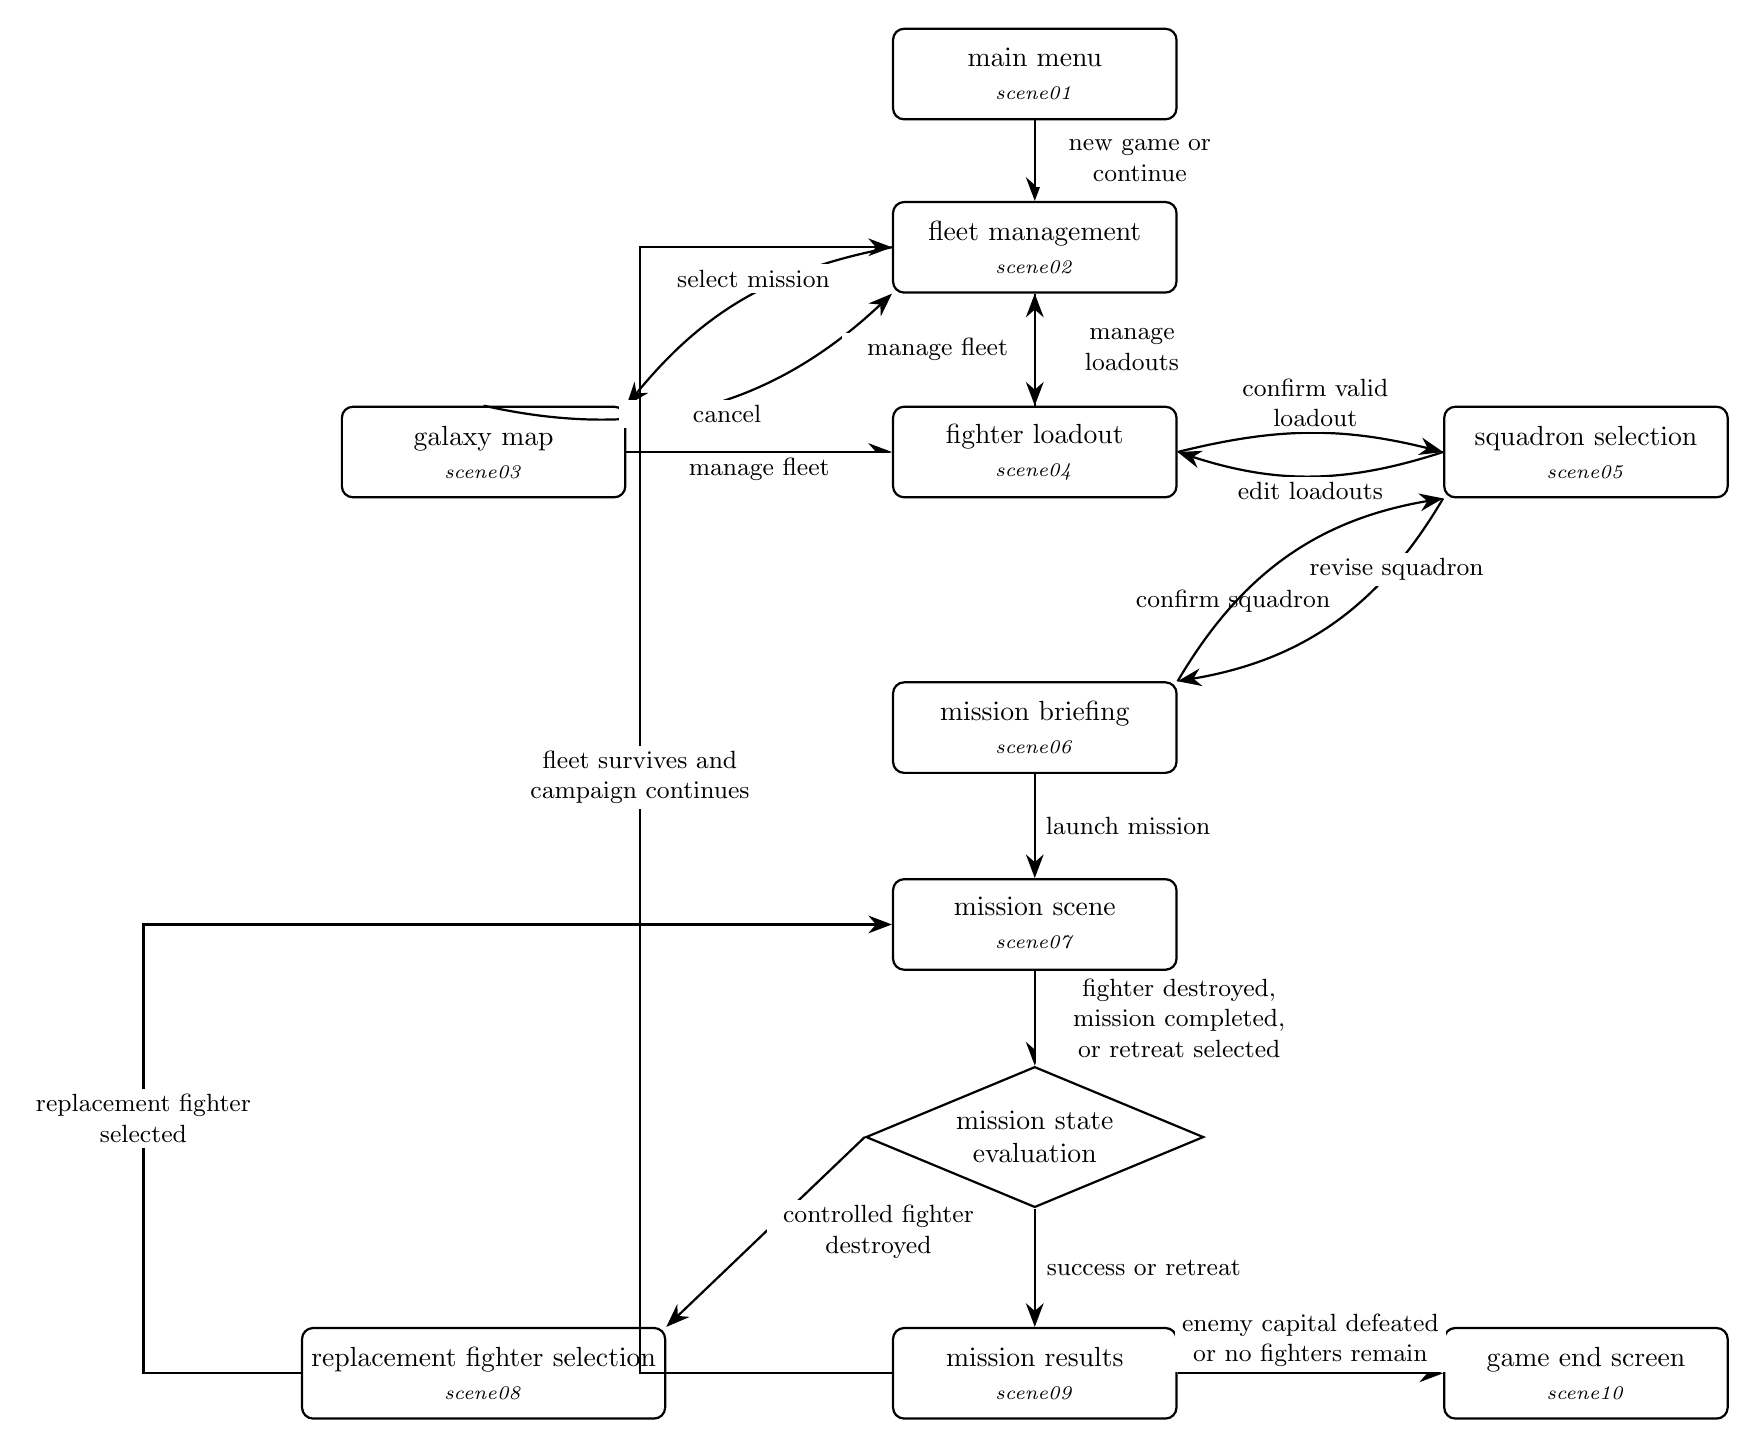
\begin{tikzpicture}[
    scene/.style={
        rectangle,
        rounded corners,
        draw,
        thick,
        align=center,
        minimum width=3.6cm,
        minimum height=1.15cm
    },
    decision/.style={
        diamond,
        draw,
        thick,
        align=center,
        aspect=2.4,
        inner sep=3pt
    },
    arrow/.style={
        -{Stealth[length=3mm]},
        thick
    },
    transition/.style={
        font=\small,
        align=center,
        fill=white,
        inner sep=2pt,
        text width=3.0cm
    }
]

% scenes

\node[scene] (menu) at (0,0) {
    main menu\\
    \scenenumber{scene01}
};

\node[scene] (fleet) at (0,-2.2) {
    fleet management\\
    \scenenumber{scene02}
};

\node[scene] (map) at (-7,-4.8) {
    galaxy map\\
    \scenenumber{scene03}
};

\node[scene] (loadout) at (0,-4.8) {
    fighter loadout\\
    \scenenumber{scene04}
};

\node[scene] (squadron) at (7,-4.8) {
    squadron selection\\
    \scenenumber{scene05}
};

\node[scene] (briefing) at (0,-8.3) {
    mission briefing\\
    \scenenumber{scene06}
};

\node[scene] (mission) at (0,-10.8) {
    mission scene\\
    \scenenumber{scene07}
};

\node[decision] (evaluation) at (0,-13.5) {
    mission state\\
    evaluation
};

\node[scene] (replacement) at (-7,-16.5) {
    replacement fighter selection\\
    \scenenumber{scene08}
};

\node[scene] (results) at (0,-16.5) {
    mission results\\
    \scenenumber{scene09}
};

\node[scene] (gameend) at (7,-16.5) {
    game end screen\\
    \scenenumber{scene10}
};

% main menu to fleet management

\draw[arrow]
    (menu) --
    node[
        transition,
        right,
        text width=2.5cm
    ] {
        new game or\\
        continue
    }
    (fleet);

% fleet management and galaxy map

\draw[arrow]
    (fleet.west)
    to[bend right=20]
    node[
        transition,
        above,
        pos=0.46,
        text width=2.2cm
    ] {
        select mission
    }
    (map.north east);

\draw[arrow]
    (map.north)
    to[bend right=28]
    node[
        transition,
        below,
        pos=0.56,
        text width=2.6cm
    ] {
        cancel
    }
    (fleet.south west);

% galaxy map and fighter loadout

\draw[arrow]
    (map.east) --
    node[
        transition,
        below,
        text width=3.2cm
    ] {
        manage fleet
    }
    (loadout.west);

\draw[arrow]
    (fleet) --
    node[
        transition,
        right,
        text width=2.3cm
    ] {
        manage loadouts
    }
    (loadout);

\draw[arrow]
    (loadout) --
    node[
        transition,
        left,
        text width=2.3cm
    ] {
        manage fleet
    }
    (fleet);

% fighter loadout and squadron selection

\draw[arrow]
    (loadout.east)
    to[bend left=14]
    node[
        transition,
        above,
        pos=0.52
    ] {
        confirm valid\\
        loadout
    }
    (squadron.west);

\draw[arrow]
    (squadron.west)
    to[bend left=18]
    node[
        transition,
        below,
        pos=0.50,
        text width=2.2cm
    ] {
        edit loadouts
    }
    (loadout.east);

% squadron selection and mission briefing

\draw[arrow]
    (squadron.south west)
    to[bend left=25]
    node[
        transition,
        above left,
        pos=0.48,
        text width=2.5cm
    ] {
        confirm squadron
    }
    (briefing.north east);

\draw[arrow]
    (briefing.north east)
    to[bend left=25]
    node[
        transition,
        below right,
        pos=0.53,
        text width=2.4cm
    ] {
        revise squadron
    }
    (squadron.south west);

% mission briefing and mission scene

\draw[arrow]
    (briefing) --
    node[
        transition,
        right,
        text width=2.2cm
    ] {
        launch mission
    }
    (mission);

% mission scene and mission-state evaluation

\draw[arrow]
    (mission) --
    node[
        transition,
        right,
        text width=3.5cm
    ] {
        fighter destroyed,\\
        mission completed,\\
        or retreat selected
    }
    (evaluation);

% replacement-fighter path

\draw[arrow]
    (evaluation.west) --
    node[
        transition,
        right,
        text width=2.7cm
    ] {
        controlled fighter\\
        destroyed 
    }
    (replacement.north east);

\draw[arrow]
    (replacement.west)
    -- ++(-2.0,0)
    |- node[
        transition,
        near start,
        above,
        text width=2.8cm
    ] {
        replacement fighter\\
        selected
    }
    (mission.west);

% continue current mission


% mission results

\draw[arrow]
    (evaluation) --
    node[
        transition,
        right,
        text width=2.6cm
    ] {
        success or retreat
    }
    (results);

% return to fleet management

\draw[arrow]
    (results.west)
    -- ++(-3.2,0)
    |- node[
        transition,
        near start,
        above,
        text width=3.2cm
    ] {
        fleet survives and\\
        campaign continues
    }
    (fleet.west);

% game end

\draw[arrow]
    (results.east) --
    node[
        transition,
        above,
        text width=3.3cm
    ] {
        enemy capital defeated\\
        or no fighters remain
    }
    (gameend.west);

\end{tikzpicture}%
}

\caption{Scene diagram for \emph{Fleet}.}
\label{fig:scene-flow}
\end{figure*}

\subsection{Scene List}

\subsubsection{Main Menu (Scene01)}

\begin{itemize}
    \item \textbf{Objective:} Begin a new game,
    continue a saved game, or exit.

    \item \textbf{Outgoing transitions:}
    To Scene02 when the player selects ``New Game'' or ``Continue.''

    \item \textbf{Game objects:}
    Buttons, Audio, Background

    \item \textbf{Comments:}
    The continue option will only be enabled when valid save data exists.
\end{itemize}


\subsubsection{Fleet Management (Scene02)}

\begin{itemize}
    \item \textbf{Objective:}
    Inspect the capital ship, pilots, fighters,
    resources, upgrades, and campaign status.

    \item \textbf{Outgoing transitions:}
    To Scene03 when the player selects ``Choose Mission.'' 
    To Scene04 when the player selects ``Manage Loadouts.''

    \item \textbf{Game objects:}
    Buttons, Audio, Background Art, Icon Art, Resource Manager

    \item \textbf{Comments:}
    This scene is the starting point of the basic game loop.
\end{itemize}


\subsubsection{Galaxy Map (Scene03)}

\begin{itemize}
    \item \textbf{Objective:}
    Inspect reachable systems, mission types,
    risks, rewards, and strategic effects.

    \item \textbf{Outgoing transitions:}
    To Scene04 when the player confirms an available mission.
    To Scene02 when the player cancels mission selection.

    \item \textbf{Game objects:}
    Mission Art, FTL Hyperlane record, Buttons, Audio, Background

    \item \textbf{Comments:}
    Only systems connected to the fleet's current location by an
    available hypergate may be selected. Info about mission will pop-up on mouse-over. 
\end{itemize}


\subsubsection{Fighter Loadout (Scene04)}

\begin{itemize}
    \item \textbf{Objective:}
    Place available equipment into the fighter's
    wing and fuselage bays.

    \item \textbf{Outgoing transitions:}
    To Scene05 when the player confirms at least one valid loadout.
    To Scene02 when the player cancels loadout management.

    \item \textbf{Game objects:}
    Loadout Manager, Fighter Preview, Left-Wing Bay, Fuselage Bay,
    Right-Wing Bay, Available Parts Panel, Power Display,
    Loadout Statistics Panel, and Loadout Interface.

    \item \textbf{Comments:}
    A valid loadout must satisfy geometric, inventory, capacity,
    and power constraints.
\end{itemize}


\subsubsection{Squadron Selection (Scene05)}

\begin{itemize}
    \item \textbf{Objective:}
    Assign loadouts to the
    squadron attempting the selected mission.

    \item \textbf{Outgoing transitions:}
    To Scene06 when the player confirms a valid squadron.
    To Scene04 when the player selects ``Edit Loadout.''

    \item \textbf{Game objects:}
    Buttons, Fleet Data, Loadout Data, Audio, Background

    \item \textbf{Comments:}
    A valid squadron must contain at least one figher and one valid loadout.
\end{itemize}


\subsubsection{Mission Briefing (Scene06)}

\begin{itemize}
    \item \textbf{Objective:}
    Present the mission objective, environment, anticipated resistance,
    selected squadron, and possible rewards.

    \item \textbf{Outgoing transitions:}
    To Scene07 when the player selects ``Launch Mission.''
    To Scene05 when the player selects ``Revise Squadron.''

    \item \textbf{Game objects:}
    Buttons, Mission Data, Audio, Background

    \item \textbf{Comments:}
    This scene gives the player a final opportunity to review the
    mission before committing the squadron.
\end{itemize}


\subsubsection{Mission Scene (Scene07)}

\begin{itemize}
    \item \textbf{Objective:}
    Fly a fighter, destroy enemies and objectives,
    protect wingmen, collect resources, complete the mission, or retreat.

    \item \textbf{Outgoing transitions:}
    To Scene08 when the controlled fighter is destroyed and another
    squadron fighter remains.
    To Scene09 when the mission succeeds, fails, or the player retreats.

    \item \textbf{Game objects:}
    Player Fighter, Wingman Fighters, Enemy Fighters,
    Rail Path, Environment Objects, Projectiles,
    Pickups, Camera Rig, and Mission HUD, Audio, Background

    \item \textbf{Comments:}
    Mission-state evaluation occurs within this scene and is not a
    separate Godot scene.
\end{itemize}


\subsubsection{Replacement Fighter Selection (Scene08)}

\begin{itemize}
    \item \textbf{Objective:}
    Choose another surviving fighter after the
    currently controlled fighter is destroyed.

    \item \textbf{Outgoing transitions:}
    To Scene07 when the player selects an available replacement fighter.

    \item \textbf{Game objects:}
    Fleet Data, Buttons, Background, Audio

    \item \textbf{Comments:}
    The mission resumes from its most recent checkpoint.
\end{itemize}


\subsubsection{Mission Results (Scene09)}

\begin{itemize}
    \item \textbf{Objective:}
    Summarize the mission outcome, pilot survival, fighter losses,
    salvage, resource rewards, and strategic effects.

    \item \textbf{Outgoing transitions:}
    To Scene02 when the fleet survives and the campaign continues.
    To Scene10 when the enemy capital is defeated or the fleet has
    no fighters remaining.

    \item \textbf{Game objects:}
    Buttons, Mission Data, Fleet Data, Audio, Background

    \item \textbf{Comments:}
    Persistent fleet and campaign data are updated before leaving
    this scene.
\end{itemize}


\subsubsection{Game End Screen (Scene10)}

\begin{itemize}
    \item \textbf{Objective:}
    Inform the player whether the campaign ended in victory or defeat
    and summarize the completed run.

    \item \textbf{Outgoing transitions:}
    To Scene01 when the player selects ``Return to Main Menu.''

    \item \textbf{Game objects:}
    Fleet data, Buttons, Audio, Background

    \item \textbf{Comments:}
    The displayed text and visual treatment depend on whether the
    enemy capital was defeated or the player's fleet was exhausted.
\end{itemize}
\section{Game Object List}

\subsection{Player Starfighter}

\begin{itemize}
    \item \textbf{Description:} The player's spaceship during missions
    \item \textbf{Tags:} Player 
    \item \textbf{Required Components: } User Input, Rigid Body, Sprite, Collider, Health, Weapons, Shields, Rail Movement, Animation, Audio
    \item \textbf{Associations: } Loadout
    \item \textbf{Comments: } This is the same even no matter which pilot has been chosen.
\end{itemize}

\subsection{Game State (prefab?)}

\begin{itemize}
    \item \textbf{Description:} Stores persistent information about the current campaign, including fighters, pilots, equipment, fuel, completed missions, and fleet location.
    \item \textbf{Tags:} Player 
    \item \textbf{Required Components: } User Input, Rigid Body, Sprite, Collider, Health, Weapons, Shields 
    \item \textbf{Associations: } Player
    \item \textbf{Comments: } This is the same even no matter which pilot has been chosen. Godot will be partially helping with scene management here.
\end{itemize}

\subsection{Mission Node}

\begin{itemize}
    \item \textbf{Description:} Represents a selectable mission on the galaxy map.
    \item \textbf{Required Components: } User Input, Art 
    \item \textbf{Associations: } Player, Map Manager
    \item \textbf{Comments: } May be randomly generated.
\end{itemize}

\subsection{Loadout Part}

\begin{itemize}
    \item \textbf{Description:} Represents a battery, weapon, shield generator, armor module, or cargo module that can be placed inside a fighter bay.
    \item \textbf{Required Components: } User Input, Art, Loadout Validation
    \item \textbf{Associations: } Player
    \item \textbf{Comments: } 
\end{itemize}

\subsection{Enemy Starfighter}

\begin{itemize}
    \item \textbf{Description:} Enemy starships
    \item \textbf{Required Components: } Rigid Body, Sprite, Collider, Health, Weapons, Shields, Movement, Animation, Audio
    \item \textbf{Comments: } There will be multiple types of art and behavior.
\end{itemize}

\subsection{Environment Object}

\begin{itemize}
    \item \textbf{Description:} Asteroids, Buildings, other obstacles
    \item \textbf{Required Components: } Rigid Body, Sprite, Collider, Animation
    \item \textbf{Comments: } None
\end{itemize}

\subsection{Laser}

\begin{itemize}
    \item \textbf{Description:} Projectile fired by player or enemy. 
    \item \textbf{Required Components: } Mesh, Collision, Movement, Damage value
    \item \textbf{Comments: } None
\end{itemize}\

\subsection{Torpedo}

\begin{itemize}
    \item \textbf{Description:} Homing Projectile fired by player
    \item \textbf{Required Components: } Mesh, Collision, Movement, Damage value
    \item \textbf{Comments: } None
\end{itemize}

\subsection{Bomb}

\begin{itemize}
    \item \textbf{Description:} Weapon fired by player
    \item \textbf{Required Components: } Area of affect, Movement, Damage value
    \item \textbf{Comments: } Is it going to have art? Or just explode?
\end{itemize}

\subsection{Pickup}

\begin{itemize}
    \item \textbf{Description:} Salvage or energy pickup by player after destroying enemy
    \item \textbf{Required Components: } Art Mesh, Collision, Cargo Capacity of Player
    \item \textbf{Comments: } None
\end{itemize}

\subsection{Camera Rig (prefab)}

\begin{itemize}
    \item \textbf{Description:} Contains the mission camera and follows the level's rail path while tracking the player's fighter.
    \item \textbf{Required Components: } 
    \item \textbf{Comments: } None
\end{itemize}

\subsection{Mission HUD}

\begin{itemize}
    \item \textbf{Description:} Displays shields, armor, energy, ammunition, cargo, squadron status, targeting information, and mission objectives.
    \item \textbf{Required Components: } Game Data
    \item \textbf{Comments: } None
\end{itemize}

\section{Component List}

\subsection{Components Provided by Godot}

\begin{itemize}

    \item \textbf{Node3D:}
    Stores three-dimensional position, rotation, and scale.

    \item \textbf{MeshInstance3D:}
    Displays a three-dimensional mesh and its materials.

    \item \textbf{CharacterBody3D:}
    Provides controlled movement and collision handling for fighters.

    \item \textbf{Area3D:}
    Detects overlapping objects such as projectiles and pickups.

    \item \textbf{CollisionShape3D:}
    Defines the collision geometry used by a physics object.

    \item \textbf{Camera3D:}
    Provides the player's view of the three-dimensional environment.

    \item \textbf{Path3D:}
    Stores the curve used for a mission rail or enemy flight path.

    \item \textbf{PathFollow3D:}
    Moves an object along a Path3D curve.

    \item \textbf{AnimationPlayer:}
    Plays named animations for fighters, equipment, and interfaces.

    \item \textbf{AudioStreamPlayer:}
    Plays music and non-positional interface audio.

    \item \textbf{AudioStreamPlayer3D:}
    Plays positional engine, weapon, impact, and explosion sounds.

    \item \textbf{Control:}
    Provides the base object for user-interface elements.

    \item \textbf{Button:}
    Provides a clickable user-interface control.

    \item \textbf{Label:}
    Displays text in menus and the mission HUD.

    \item \textbf{TextureRect:}
    Displays interface icons, portraits, and backgrounds.

    \item \textbf{ProgressBar:}
    Displays continuous values such as shields and energy.

\end{itemize}

\subsection{Minimum Required Custom Components}

\begin{itemize}

    \item \textbf{Scene Navigation:}
    Changes scenes when the appropriate button is selected or gameplay condition is satisfied.

    \item \textbf{Game State:}
    Preserves fleet and campaign information between scenes.

    \item \textbf{Fleet Inventory:}
    Tracks available fighters, equipment, fuel, resources, and salvage.

    \item \textbf{Player Input:}
    Converts keyboard or controller input into movement, aiming, firing, maneuvers, and menu commands.

    \item \textbf{Rail Movement:}
    Advances the player and camera along a predefined path while limiting the fighter to the playable area.

    \item \textbf{Maneuver:}
    Performs boosting, braking, barrel rolls, somersaults, and hard banks while enforcing energy costs.

    \item \textbf{Energy:}
    Tracks powerplant output, battery capacity, current energy, recharge, and energy consumption.

    \item \textbf{Weapon:}
    Stores damage, firing rate, projectile type, ammunition, and energy cost.

    \item \textbf{Shield:}
    Absorbs damage, consumes energy, recharges, and reports its status to the HUD.

    \item \textbf{Armor:}
    Determines how many unshielded hits a fighter can survive.

    \item \textbf{Damage:}
    Receives damage and reports when an object or fighter has been destroyed.

    \item \textbf{Cargo:}
    Tracks collected salvage and prevents collection beyond maximum capacity.

    \item \textbf{Pickup:}
    Applies the effect of an energy or salvage object when collected.

    \item \textbf{Projectile Movement:}
    Moves a projectile, detects impacts, and removes it after its lifetime
    expires.

    \item \textbf{Enemy Flight AI:}
    Moves an enemy along an attack path and selects opportunities to fire.

    \item \textbf{Mission Controller:}
    Advances encounters, checks objectives, stores checkpoints, and determines mission outcomes.

    \item \textbf{Spawn Controller:}
    Creates enemies, obstacles, and pickups at predefined locations.

    \item \textbf{Objective Tracker:}
    Tracks whether mission targets have been destroyed, reached, protected, or survived.

    \item \textbf{Squadron State:}
    Tracks deployed fighters and determines whether a replacement remains.

    \item \textbf{Loadout Validation:}
    Checks equipment geometry, availability, capacity, and power requirements.

    \item \textbf{HUD Presenter:}
    Reads gameplay values and updates the mission HUD.

\end{itemize}


\subsection{Stretch-Goal Custom Components}

\begin{itemize}

    \item \textbf{Target Lock:}
    Selects a target and determines when a torpedo lock has been acquired.

    \item \textbf{Homing Guidance:}
    Rotates a torpedo toward its selected target.

    \item \textbf{Area Damage:}
    Applies bomb or explosion damage within a specified radius.

    \item \textbf{Sectional Damage:}
    Tracks damage to the fuselage and each wing separately.

    \item \textbf{Wingman AI:}
    Allows allied fighters to attack, evade, and respond to danger.

    \item \textbf{Threat and Rescue:}
    Identifies endangered wingmen and tracks whether the player rescues them.

    \item \textbf{Tow Recovery:}
    Calculates whether a disabled fighter and its escorts return successfully.

    \item \textbf{Pilot Legend:}
    Stores pilot victories, survival, prestige, and accomplishments.

    \item \textbf{Ace Persistence:}
    Stores whether a named enemy ace survives to appear in later missions.

    \item \textbf{Strategic Impact:}
    Applies mission results to enemy fuel, defense, and industrial strength.

    \item \textbf{Encounter Variation:}
    Selects alternate enemy groups and obstacle arrangements.

\end{itemize}


\section{Visual Assets List}

\subsection{Minimum Custom Visual Assets}

\begin{itemize}

    \item \textbf{Capsule Art:}
    A static title image showing the capital ship and its fighters.

    \item \textbf{Player Fighter:}
    A low-poly animated model stored as a Blockbench source file and exported as a GLB file. It will include the following local animation sequences:
    \begin{itemize}
        \item \texttt{boost}: engine vanes open and engine glow increases;
        \item \texttt{brake}: braking panels extend from the fighter;
        \item \texttt{fire}: muzzle flashes on the ship
    \end{itemize}

    \item \textbf{Enemy Fighter:}
    A static low-poly model with a silhouette distinct from the player fighter. It will be stored as a Blockbench file and exported as GLB.

    \item \textbf{Capital Ship:}
    A static low-poly exterior model used in fleet management and mission backgrounds. It will be exported as GLB.

    \item \textbf{Projectiles and Pickups:}
    Static laser, energy-sphere, and salvage models exported as GLB files.

    \item \textbf{Asteroid Set:}
    Asteroid models of different sizes and shapes.

    \item \textbf{Buildings}
    Building models of different sizes and shapes.

    \item \textbf{Mission Target:}
    A static defense satellite or station,  used as the objective of the minimum mission.

    \item \textbf{Space Environment:}
    A static star field, distant planet, defense satellite and nebula stored as PNG files

    \item \textbf{Interface Assets:}
    Static icons for shields, armor, energy, weapons, cargo, fuel, fighters, and mission objectives. Source files will be SVG or PNG.

\end{itemize}

\subsection{Stretch Goal Visual Assets}

\begin{itemize}

    \item Interceptor, bomber, and enemy-ace models.
    \item Turrets, defense satellites, and an enemy capital ship.
    \item Bomb and homing-torpedo models.
    \item Animated hypergate structures and travel effects.
    \item Fighter wrecks, detached wings, smoke, sparks, and damaged materials.
    \item Gas-giant, asteroid-field, orbital, planetary, and capital environments.
    \item Pilot portraits, names, insignia, and legend markers.
    \item Shield impacts, explosions, engine trails, and targeting effects.

\end{itemize}


\section{Audio Assets List}

Audio assets will be edited in Audacity and stored in the usual format. (I am not sure what that is.)

\subsection{Minimum Custom Audio Assets}

\begin{itemize}

    \item \textbf{Mission Theme:}
    Looping stereo music played during the minimum combat mission.

    \item \textbf{Fighter Engine:}
    A looping mono sound whose pitch changes during boosting and braking.

    \item \textbf{Laser Fire:}
    A short mono sound played whenever a laser is fired.

    \item \textbf{Shield Impact:}
    An electronic sound played when a shield absorbs damage.


    \item \textbf{Explosion:}
    A sound played when a fighter, asteroid, or mission target is destroyed.

    \item \textbf{Energy Pickup:}
    A rising tone played when the player collects energy.

    \item \textbf{Salvage Pickup:}
    A mechanical confirmation sound played when salvage is collected.

    \item \textbf{Interface Confirmation:}
    A short sound played when a menu option is selected.

\end{itemize}


\subsection{Stretch Goal Full-Game Audio Assets}

\begin{itemize}

    \item Fleet-management and galaxy-map music.
    \item Boss, victory, and defeat themes.
    \item Torpedo lock, launch, flight, and impact sounds.
    \item Bomb launch and explosion sounds.
    \item Wingman radio messages and rescue requests.
    \item Hypergate activation and travel sounds.
    \item Low-shield, low-energy, damage, and retreat warnings.

\end{itemize}


\section{Team Tasks}

\subsection{Minimum Required Tasks}

\begin{itemize}

    \item \textbf{Taylor, July 10--12:}
    Finalize the design document, establish the Godot project, and maintain the GitHub repository.

    \item \textbf{Taylor and Clayton, July 10--14:}
    Establish the low-poly visual style and review concept art.

    \item \textbf{Clayton, July 15--24:}
    Assist with selected models, visual feedback, and playtesting.

    \item \textbf{Taylor and Clayton, July 25--29:}
    Conduct structured playtests and identify control, interface, and balance problems.

    \item \textbf{Taylor, July 30--31:}
    Prepare the final build, documentation, demonstration, and submission.

\end{itemize}


\subsection{Full-Game Tasks}

After the minimum build is stable, Taylor and Clayton will select additional enemy types, missions, art assets, and strategic systems to complete as time permits.


\section{Programming Tasks}

\subsection{Minimum Programming Tasks}

\begin{itemize}

    \item \textbf{July 10--14, Taylor:}
    Implement scene navigation, persistent game state, player movement, rail movement, camera behavior, and input.

    \item \textbf{July 15--18, Taylor:}
    Implement weapons, enemies, asteroids, collisions, shields, armor, energy,  destruction, and pickups.

    \item \textbf{July 19--22, Taylor:}
    Implement fighter loadouts, fleet inventory, squadron selection, and replacement fighters.

    \item \textbf{July 23--25, Taylor:}
    Implement mission objectives, checkpoints, retreat, mission results, game failure, and the minimum galaxy map.

    \item \textbf{July 26--28, Taylor:}
    Integrate menus, the HUD, visual assets, animation, audio, and save data.

    \item \textbf{July 29--31, Taylor:}
    Correct critical defects, balance the mission, optimize performance, and export the final build.

\end{itemize}


\subsection{Full-Game Programming Tasks}

Full-game programming may include wingman AI, bombs, homing torpedoes, sectional damage, towing, named enemy aces, pilot legends, additional mission types, strategic consequences, and the final enemy-capital mission. 


\section{Art Tasks}

\subsection{Minimum Required Art Tasks}

\begin{itemize}

    \item \textbf{July 10--13, Taylor and Clayton:}
    Produce capsule art and interface concept art.

    \item \textbf{July 12--18, Taylor and Clayton:}
    Model the player fighter, enemy fighter, capital ship, asteroids, mission target, projectiles, and pickups. Create sound effects and mission track music.

    \item \textbf{July 16--21, Taylor and Clayton:}
    Create boost, brake, and wing-damage animations. Create sound effects and mission track music.

    \item \textbf{July 19--24, Taylor and Clayton:}
    Create interface icons, materials, backgrounds, and particle effects. Create sound effects and mission track music.

    \item \textbf{July 25--28, Taylor and Clayton:}
    Review asset consistency, readability, scale, and appearance in Godot. 

\end{itemize}


\subsection{Full-Game Art Tasks}

Full-game art may include additional fighter classes, enemy aces, turrets, capital ships, hypergates, planetary structures, pilot portraits, wrecks, damage states, and additional mission environments. Additional tracks for types of missions and menus.

\section{Testing Tasks}

\subsection{Minimum Testing Tasks}

\begin{itemize}

    \item \textbf{July 14--22, Taylor:}
    Test movement, firing, collisions, energy, shields, armor, pickups, and loadout validation as they are implemented.

    \item \textbf{July 23--27, Taylor:}
    Test all scene transitions and verify that fleet and campaign data persist.

    \item \textbf{July 25--29, Taylor and Clayton:}
    Conduct playtests focused on controls, objective clarity, interface readability, mission length, and difficulty.

    \item \textbf{July 29--30, Taylor:}
    Test victory, failure, retreat, replacement-fighter, save, load, and game-end conditions.

    \item \textbf{July 31, Taylor:}
    Perform a final test and correct crashes, soft locks, and
    progression blockers.

\end{itemize}


\subsection{Full-Game Testing Tasks}

Any full-game feature will receive functional and integration testing before
being included. Features that create crashes, progression blockers, or major
balance problems will be removed from the submitted build.

\section{Original Concept Art}

\begin{figure}[h]
    \centering
    \includegraphics[width=\linewidth]{fighter_sketch.jpg}
    \caption{Starfighter Pen Sketch From above and behind}
    \label{fig:fighter sketch}
\end{figure}

\begin{figure}[h]
    \centering
    \includegraphics[width=\linewidth]{fighter_sketch2.jpg}
    \caption{Starfighter Pen Sketch From the side and behind}
    \label{fig:fighter sketch}
\end{figure}

\begin{figure}[h]
    \centering
    \includegraphics[width=\linewidth]{fightermodel2.png}
    \caption{Starfighter Model}
    \label{fig:fighter sketch}
\end{figure}

\begin{figure}[h]
    \centering
    \includegraphics[width=\linewidth]{capital_sketch.jpg}
    \caption{Capital Ship Pen Sketch}
    \label{fig:capital ship sketch}
\end{figure}


\end{document}